%        File: arfc-beamer.tex
%     Created: Sun May 5 10:00 PM 2013 C
%


%\documentclass[11pt,handout]{beamer}
\documentclass[9pt]{beamer}
\usetheme[white]{Illinois}
%\title[short title]{long title}
\title[Cyclus, an agent-based fuel cycle simulator]{Cyclus, an agent-based fuel cycle simulator}
%\subtitle[short subtitle]{long subtitle}
\subtitle[Brief Overview]{Brief Overview}
%\author[short name]{long name}
\author[Jin Whan Bae, Kathryn Huff]{Jin Whan Bae, Kathryn Huff}
%\date[short date]{long date}
\date[05.21.2018]{May 21, 2018}
%\institution[short name]{long name}
\institute[UIUC]{University of Illinois at Urbana-Champaign}

%%%% Acronym support

\usepackage[acronym,toc]{glossaries}
%\newacronym{<++>}{<++>}{<++>}
\newacronym{ABM}{ABM}{agent-based modeling}
\newacronym{ACDIS}{ACDIS}{Program in Arms Control \& Domestic and International Security}
\newacronym{ADS}{ADS}{Accelerator-Driven Systems}
\newacronym{AHTR}{AHTR}{Advanced High Temperature Reactor}
\newacronym{ANDRA}{ANDRA}{Agence Nationale pour la gestion des D\'echets RAdioactifs, the French National Agency for Radioactive Waste Management}
\newacronym{ANL}{ANL}{Argonne National Laboratory}
\newacronym{ANS}{ANS}{American Nuclear Society}
\newacronym{API}{API}{application programming interface}
\newacronym{ARE}{ARE}{Aircraft Reactor Experiment}
\newacronym{ARFC}{ARFC}{Advanced Reactors and Fuel Cycles}
\newacronym{ASME}{ASME}{American Society of Mechanical Engineers}
\newacronym{ATWS}{ATWS}{Anticipated Transient Without Scram}
\newacronym{BDBE}{BDBE}{Beyond Design Basis Event}
\newacronym{BIDS}{BIDS}{Berkeley Institute for Data Science}
\newacronym{BWR}{BWR}{Boiling Water Reactor}
\newacronym{CAFCA}{CAFCA}{ Code for Advanced Fuel Cycles Assessment }
\newacronym{CDTN}{CDTN}{Centro de Desenvolvimento da Tecnologia Nuclear}
\newacronym{CEA}{CEA}{Commissariat \`a l'\'Energie Atomique et aux \'Energies Alternatives}
\newacronym{CI}{CI}{continuous integration}
\newacronym{CNEN}{CNEN}{Comiss\~{a}o Nacional de Energia Nuclear}
\newacronym{CNERG}{CNERG}{Computational Nuclear Engineering Research Group}
\newacronym{COSI}{COSI}{Commelini-Sicard}
\newacronym{COTS}{COTS}{commercial, off-the-shelf}
\newacronym{CSNF}{CSNF}{commercial spent nuclear fuel}
\newacronym{CTAH}{CTAHs}{Coiled Tube Air Heaters}
\newacronym{CUBIT}{CUBIT}{CUBIT Geometry and Mesh Generation Toolkit}
\newacronym{CURIE}{CURIE}{Centralized Used Fuel Resource for Information Exchange}
\newacronym{DAG}{DAG}{directed acyclic graph}
\newacronym{DANESS}{DANESS}{Dynamic Analysis of Nuclear Energy System Strategies}
\newacronym{DBE}{DBE}{Design Basis Event}
\newacronym{DESAE}{DESAE}{Dynamic Analysis of Nuclear Energy Systems Strategies}
\newacronym{DHS}{DHS}{Department of Homeland Security}
\newacronym{DOE}{DOE}{Department of Energy}
\newacronym{DRACS}{DRACS}{Direct Reactor Auxiliary Cooling System}
\newacronym{DRE}{DRE}{dynamic resource exchange}
\newacronym{DSNF}{DSNF}{DOE spent nuclear fuel}
\newacronym{DYMOND}{DYMOND}{Dynamic Model of Nuclear Development }
\newacronym{EBS}{EBS}{Engineered Barrier System}
\newacronym{EDF}{EDF}{\`{E}lectricit\`{e} de France}
\newacronym{EDZ}{EDZ}{Excavation Disturbed Zone}
\newacronym{EIA}{EIA}{U.S. Energy Information Administration}
\newacronym{EPA}{EPA}{Environmental Protection Agency}
\newacronym{EPR}{EPR}{European Pressurized Reactor}
\newacronym{EP}{EP}{Engineering Physics}
\newacronym{EU}{EU}{European Union}
\newacronym{FCO}{FCO}{Fuel Cycle Options}
\newacronym{FCT}{FCT}{Fuel Cycle Technology}
\newacronym{FEHM}{FEHM}{Finite Element Heat and Mass Transfer}
\newacronym{FEPs}{FEPs}{Features, Events, and Processes}
\newacronym{FHR}{FHR}{Fluoride-Salt-Cooled High-Temperature Reactor}
\newacronym{FLiBe}{FLiBe}{Fluoride-Lithium-Beryllium}
\newacronym{FP}{FP}{Fission Products}
\newacronym{GDSE}{GDSE}{Generic Disposal System Environment}
\newacronym{GDSM}{GDSM}{Generic Disposal System Model}
\newacronym{GENIUSv1}{GENIUSv1}{Global Evaluation of Nuclear Infrastructure Utilization Scenarios, Version 1}
\newacronym{GENIUSv2}{GENIUSv2}{Global Evaluation of Nuclear Infrastructure Utilization Scenarios, Version 2}
\newacronym{GENIUS}{GENIUS}{Global Evaluation of Nuclear Infrastructure Utilization Scenarios}
\newacronym{GPAM}{GPAM}{Generic Performance Assessment Model}
\newacronym{GRSAC}{GRSAC}{Graphite Reactor Severe Accident Code}
\newacronym{GUI}{GUI}{graphical user interface}
\newacronym{HLW}{HLW}{high level waste}
\newacronym{HPC}{HPC}{high-performance computing}
\newacronym{HTC}{HTC}{high-throughput computing}
\newacronym{HTGR}{HTGR}{High Temperature Gas-Cooled Reactor}
\newacronym{IAEA}{IAEA}{International Atomic Energy Agency}
\newacronym{IEMA}{IEMA}{Illinois Emergency Mangament Agency}
\newacronym{IHLRWM}{IHLRWM}{International High Level Radioactive Waste Management}
\newacronym{INL}{INL}{Idaho National Laboratory}
\newacronym{IPRR1}{IRP-R1}{Instituto de Pesquisas Radioativas Reator 1}
\newacronym{IRP}{IRP}{Integrated Research Project}
\newacronym{ISFSI}{ISFSI}{Independent Spent Fuel Storage Installation}
\newacronym{ISRG}{ISRG}{Independent Student Research Group}
\newacronym{JFNK}{JFNK}{Jacobian-Free Newton Krylov}
\newacronym{LANL}{LANL}{Los Alamos National Laboratory}
\newacronym{LBNL}{LBNL}{Lawrence Berkeley National Laboratory}
\newacronym{LCOE}{LCOE}{levelized cost of electricity}
\newacronym{LDRD}{LDRD}{laboratory directed research and development}
\newacronym{LFR}{LFR}{Lead-Cooled Fast Reactor}
\newacronym{LLNL}{LLNL}{Lawrence Livermore National Laboratory}
\newacronym{LMFBR}{LMFBR}{Liquid Metal Fast Breeder Reactor}
\newacronym{LOFC}{LOFC}{Loss of Forced Cooling}
\newacronym{LOHS}{LOHS}{Loss of Heat Sink}
\newacronym{LOLA}{LOLA}{Loss of Large Area}
\newacronym{LP}{LP}{linear program}
\newacronym{LWR}{LWR}{Light Water Reactor}
\newacronym{MAGNOX}{MAGNOX}{Magnesium Alloy Graphie Moderated Gas Cooled Uranium Oxide Reactor}
\newacronym{MA}{MA}{minor actinide}
\newacronym{MCNP}{MCNP}{Monte Carlo N-Particle code}
\newacronym{MILP}{MILP}{mixed-integer linear program}
\newacronym{MIT}{MIT}{the Massachusetts Institute of Technology}
\newacronym{MOAB}{MOAB}{Mesh-Oriented datABase}
\newacronym{MOOSE}{MOOSE}{Multiphysics Object-Oriented Simulation Environment}
\newacronym{MOX}{MOX}{mixed oxide}
\newacronym{MSBR}{MSBR}{Molten Salt Breeder Reactor}
\newacronym{MSRE}{MSRE}{Molten Salt Reactor Experiment}
\newacronym{MSR}{MSR}{Molten Salt Reactor}
\newacronym[longplural={metric tons of heavy metal}]{MTHM}{MTHM}{metric ton of heavy metal}
\newacronym{NAGRA}{NAGRA}{National Cooperative for the Disposal of Radioactive Waste}
\newacronym{NEAMS}{NEAMS}{Nuclear Engineering Advanced Modeling and Simulation}
\newacronym{NEUP}{NEUP}{Nuclear Energy University Programs}
\newacronym{NFCSim}{NFCSim}{Nuclear Fuel Cycle Simulator}
\newacronym{NGNP}{NGNP}{Next Generation Nuclear Plant}
\newacronym{NMWPC}{NMWPC}{Nuclear MW Per Capita}
\newacronym{NNSA}{NNSA}{National Nuclear Security Administration}
\newacronym{NPRE}{NPRE}{Department of Nuclear, Plasma, and Radiological Engineering}
\newacronym{NQA1}{NQA-1}{Nuclear Quality Assurance - 1}
\newacronym{NRC}{NRC}{Nuclear Regulatory Commission}
\newacronym{NSF}{NSF}{National Science Foundation}
\newacronym{NSSC}{NSSC}{Nuclear Science and Security Consortium}
\newacronym{NUWASTE}{NUWASTE}{Nuclear Waste Assessment System for Technical Evaluation}
\newacronym{NWF}{NWF}{Nuclear Waste Fund}
\newacronym{NWTRB}{NWTRB}{Nuclear Waste Technical Review Board}
\newacronym{OCRWM}{OCRWM}{Office of Civilian Radioactive Waste Management}
\newacronym{ORION}{ORION}{ORION}
\newacronym{ORNL}{ORNL}{Oak Ridge National Laboratory}
\newacronym{PARCS}{PARCS}{Purdue Advanced Reactor Core Simulator}
\newacronym{PBAHTR}{PB-AHTR}{Pebble Bed Advanced High Temperature Reactor}
\newacronym{PBFHR}{PB-FHR}{Pebble-Bed Fluoride-Salt-Cooled High-Temperature Reactor}
\newacronym{PEI}{PEI}{Peak Environmental Impact}
\newacronym{PH}{PRONGHORN}{PRONGHORN}
\newacronym{PRIS}{PRIS}{Power Reactor Information System}
\newacronym{PRKE}{PRKE}{Point Reactor Kinetics Equations}
\newacronym{PSPG}{PSPG}{Pressure-Stabilizing/Petrov-Galerkin}
\newacronym{PWAR}{PWAR}{Pratt and Whitney Aircraft REeactor}
\newacronym{PWR}{PWR}{Pressurized Water Reactor}
\newacronym{PyNE}{PyNE}{Python toolkit for Nuclear Engineering}
\newacronym{PyRK}{PyRK}{Python for Reactor Kinetics}
\newacronym{QA}{QA}{quality assurance}
\newacronym{RDD}{RD\&D}{Research Development and Demonstration}
\newacronym{RD}{R\&D}{Research and Development}
\newacronym{RELAP}{RELAP}{Reactor Excursion and Leak Analysis Program}
\newacronym{RIA}{RIA}{Reactivity Insertion Accident}
\newacronym{RIF}{RIF}{Region-Institution-Facility}
\newacronym{SFR}{SFR}{Sodium-Cooled Fast Reactor}
\newacronym{SINDAG}{SINDA{\textbackslash}G}{Systems Improved Numerical Differencing Analyzer $\backslash$ Gaski}
\newacronym{SKB}{SKB}{Svensk K\"{a}rnbr\"{a}nslehantering AB}
\newacronym{SNF}{SNF}{spent nuclear fuel}
\newacronym{SNL}{SNL}{Sandia National Laboratory}
\newacronym{STC}{STC}{specific temperature change}
\newacronym{SUPG}{SUPG}{Streamline-Upwind/Petrov-Galerkin}
\newacronym{SWF}{SWF}{Separations and Waste Forms}
\newacronym{SWU}{SWU}{Separative Work Unit}
\newacronym{ThOX}{ThOX}{thorium oxide}
\newacronym{TRIGA}{TRIGA}{Training Research Isotope General Atomic}
\newacronym{TRISO}{TRISO}{Tristructural Isotropic}
\newacronym{TSM}{TSM}{Total System Model}
\newacronym{TSPA}{TSPA}{Total System Performance Assessment for the Yucca Mountain License Application}
\newacronym{UFD}{UFD}{Used Fuel Disposition}
\newacronym{UML}{UML}{Unified Modeling Language}
\newacronym{UNF}{UNF}{Used Nuclear Fuel}
\newacronym{UOX}{UOX}{uranium oxide}
\newacronym{UQ}{UQ}{uncertainty quantification}
\newacronym{US}{US}{United States}
\newacronym{UW}{UW}{University of Wisconsin}
\newacronym{VISION}{VISION}{the Verifiable Fuel Cycle Simulation Model}
\newacronym{VVER}{VVER}{Voda-Vodyanoi Energetichesky Reaktor (Russian Pressurized Water Reactor)}
\newacronym{VV}{V\&V}{verification and validation}
\newacronym{WIPP}{WIPP}{Waste Isolation Pilot Plant}
\newacronym{YMR}{YMR}{Yucca Mountain Repository Site}


\makeglossaries

%\usepackage{bbding}
\usepackage{amsfonts}
\usepackage{adjustbox}
\usepackage{fancyvrb}
\usepackage{amsmath}
\usepackage{xspace}
\usepackage{graphicx}
\usepackage{subfigure}
\usepackage{listings}
\usepackage{booktabs} % nice rules for tables
\usepackage{microtype} % if using PDF
\usepackage{bigints}
\DeclareMathOperator{\erf}{erf}
%I need some complimentary error funcitons... 
\DeclareMathOperator{\erfc}{erfc}
%page numbers
\setbeamertemplate{footline}[page number]
\setbeamertemplate{caption}[numbered]
%Those icons in the references are terrible looking
\setbeamertemplate{bibliography item}[text]


%try to get rid of header on title page\dots
\makeatletter
    \newenvironment{withoutheadline}{
        \setbeamertemplate{headline}[default]
        \def\beamer@entrycode{\vspace*{-\headheight}}
    }{}
\makeatother


\usepackage{booktabs} % nice rules (thick lines) for tables
\usepackage{microtype} % improves typography for PDF
\usepackage{xspace}
\usepackage{tabularx}
\usepackage[affil-it]{authblk}
\usepackage{tikz}

\usepackage{tikz}
\usetikzlibrary{positioning, arrows, decorations, shapes}

\usetikzlibrary{shapes.geometric,arrows}
\tikzstyle{process} = [rectangle, rounded corners, minimum width=3cm, minimum height=1cm,text centered, draw=black, fill=blue!30]
\tikzstyle{object} = [ellipse, rounded corners, minimum width=3cm, minimum height=1cm,text centered, draw=black, fill=green!30]
\tikzstyle{arrow} = [thick,->,>=stealth]

\usepackage{cleveref}
\usepackage{datatool}
\newcolumntype{b}{X}
\newcolumntype{s}{>{\hsize=.5\hsize}X}
\newcolumntype{m}{>{\hsize=.75\hsize}X}

\newcommand{\Cyclus}{\textsc{Cyclus}\xspace}%
\graphicspath{ {images/} }
\usetikzlibrary{positioning, arrows, decorations, shapes }

\begin{document}
%%%%%%%%%%%%%%%%%%%%%%%%%%%%%%%%%%%%%%%%%%%%%%%%%%%%%%%%%%%%%
%% From uw-beamer Here's a handy bit of code to place at 
%% the beginning of your presentation (after \begin{document}):
\newcommand*{\alphabet}{ABCDEFGHIJKLMNOPQRSTUVWXYZabcdefghijklmnopqrstuvwxyz}
\newlength{\highlightheight}
\newlength{\highlightdepth}
\newlength{\highlightmargin}
\setlength{\highlightmargin}{2pt}
\settoheight{\highlightheight}{\alphabet}
\settodepth{\highlightdepth}{\alphabet}
\addtolength{\highlightheight}{\highlightmargin}
\addtolength{\highlightdepth}{\highlightmargin}
\addtolength{\highlightheight}{\highlightdepth}
\newcommand*{\Highlight}{\rlap{\textcolor{HighlightBackground}{\rule[-\highlightdepth]{\linewidth}{\highlightheight}}}}
%%%%%%%%%%%%%%%%%%%%%%%%%%%%%%%%%%%%%%%%%%%%%%%%%%%%%%%%%%%%%
%%--------------------------------%%
\begin{withoutheadline}
\frame{
  \titlepage
}
\end{withoutheadline}

%%--------------------------------%%

\section{Before We Start}
\begin{frame}
	\frametitle{Agent-based Framework}
	\begin{itemize}
		\item Cyclus is agent-based, which means it's very modular
		\item User can develop / plug in facilities
			\begin{itemize}
				\item User can `design' their own fuel cycle
				\item Highly customizable
			\end{itemize}
	\end{itemize}
	\begin{figure}[htbp!]
        \begin{center}
                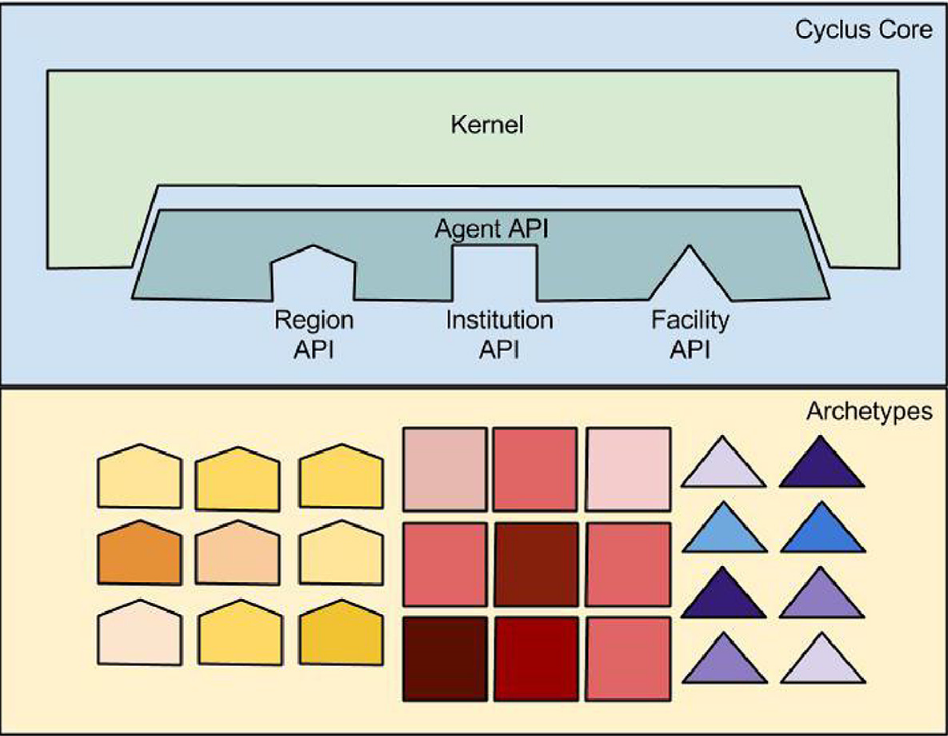
\includegraphics[width=.6\textwidth]{./images/cyclus_structure.png}
        \end{center}
        \caption{Modular Design of Cyclus}
        \label{fig:cyclus_struc}

	\end{figure}
\end{frame}

\begin{frame}
    \frametitle{Timestep Execution}
    A simplified explanation: Each timestep:
    
\begin{figure}[H]
\centering
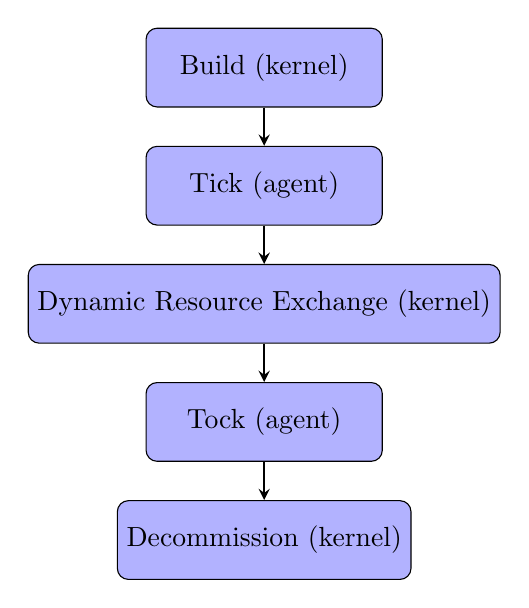
\begin{tikzpicture}[node distance=1.5cm]
\node (Build) [process] {Build (kernel)};
\node (Tick) [process, below of=Build] {Tick (agent)};
\node (DRE) [process, below of=Tick]{Dynamic Resource Exchange (kernel) };
\node (Tock) [process, below of=DRE]{Tock (agent)};
\node (Decom) [process, below of=Tock] {Decommission (kernel)};

\draw [arrow] (Build) -- (Tick); 
\draw [arrow] (Tick) -- (DRE);
\draw [arrow] (DRE) -- (Tock);
\draw [arrow] (Tock) -- (Decom);
\end{tikzpicture}
\end{figure}

\end{frame}

\begin{frame}
	\frametitle{General Info}
	\begin{itemize}
		\item Written in: C++, Python
		\item Input file: xml, json, python
		\item Output file: .sqlite, .hdf5
	\end{itemize}
\end{frame}


\begin{frame}
	\frametitle{Terminology}
	\begin{itemize}
		\item \textbf{Archetypes}: A collection of logic and behavior which can be configured into a prototype which can then be instantiated in simulation as a agent. Archetypes are represented as C++ classes that inherit from the base cyclus::Agent class. (e.g. Reactor module, Sink module)
		\item \textbf{Prototypes}: Archetype + parameters (e.g. Reactor with input-defined  \texttt{name, cycle time, assembly size, core size etc})
		\item \textbf{Agents}: Every single `entity' in play during simulation (Region, Institution, Facility)
	\end{itemize}
\end{frame}

\begin{frame}
	\frametitle{Terminology}
	\begin{itemize}
		\item \textbf{Region}: The group agent that is a collection of institutions (Can manage / control regions)
		\item \textbf{Institution}: Agent that manages facilities (Can deploy, decommission facilities)
		\item \textbf{Facility}: The agent that `trades' and does calculations (Trades material and transmutes, separates)
	\end{itemize}
\end{frame}

\begin{frame}
	\frametitle{Extensions - Archetypes}
	Since Cyclus is an extensible framework, anyone can develop a new archetype and plug-and-play. (\textcolor{blue}{Institution}, \textcolor{red}{region}, facility otherwise.)
	\begin{itemize}
		\item Cycamore: Sink, Storage, Recipe Reactor, Fuelfab, Enrichment, Source, \textcolor{blue}{DeployInst}, Mixer, Separations, \textcolor{red}{GrowthRegion}
		\item \textcolor{blue}{d3ploy}: Demand-driven deployment Institution (NEUP 16-10512)
		\item CYBORG: Reactor depletion analysis tool using ORIGEN
		\item CYDER: A CYclus Disposal Environment and Repository object.
		\item CORRM: Continuous On-line Reprocessing Reactor Module.
		\item Pyre: Pyroprocessing module with non-proliferation metrics
		\item And more..
	\end{itemize}
\end{frame}

\begin{frame}
	\frametitle{Extensions - Analysis / Drivers}
	There are other tools to help visualization / output data analysis of Cyclus.
	\begin{itemize}
		\item RICKSHAW: Automated stochastic driver for Cyclus
		\item Cymetric: Extracts important fuel cycle metrics
		\item Analysis: Collection of functions to extract metrics (e.g. natU usage, trade between two facilities, etc.)
		\item Cycmap: GIS visualization tool for Cyclus
		\item Cyclist: GUI for Cyclus (DEPRACATED)
	\end{itemize}
\end{frame}


\begin{frame}
	\frametitle{Installation - Binary}
	Better, more thorough explanations are in \texttt{fuelcycle.org}
	\begin{itemize}
		\item Windows: N/A
		\item MacOS: \texttt{conda install -c conda-forge cyclus cycamore}
		\item Linux: \texttt{conda install cyclus cycamore}
	\end{itemize}
\end{frame}


\begin{frame}
	\frametitle{Installation - Build from Source}
    All source files are open-source, and available on Github.

	\texttt{github.com/cyclus/cyclus} and \texttt{github.com/cycamore/cycamore} has the source files, and guides
	\begin{enumerate}
		\item Clone repository (\texttt{git clone [url]})
		\item Install dependency (see github guide README)
		\item \texttt{python install.py}
	\end{enumerate}
\end{frame}


\begin{frame}
	\frametitle{Installation - TroubleShooting}
	Look for your error message or make a new post in the following Cyclus communities:
	\begin{enumerate}
		\item Github Issue in \texttt{github.com/cyclus/cyclus}
		\item Cyclus google user group
        \item Email jbae11@illinois.edu (me)
	\end{enumerate}
\end{frame}




\section{Running Simulations}
\begin{frame}
    \frametitle{Structure}
    \begin{enumerate}
        \item \texttt{Control}: Simulation Definition
        \item \texttt{Archetypes}: List of available archetypes
        \item \texttt{Facility}: Facility prototypes - define parameters of archetypes
        \item \texttt{Region}: Region agents
        \item \texttt{Institution}: Institution agents (inside Region definition)
        \item \texttt{Recipe}: recipe definitions
    \end{enumerate}
\end{frame}

\begin{frame}
    \frametitle{Control}
\begin{figure}[htbp!]
        \begin{center}
                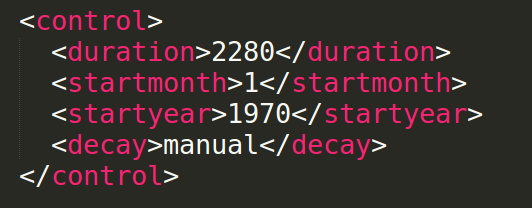
\includegraphics[width=.8\textwidth]{./images/control.png}
        \end{center}
    \end{figure}

\end{frame}

\begin{frame}
    \frametitle{Archetypes}
\begin{figure}[htbp!]
        \begin{center}
                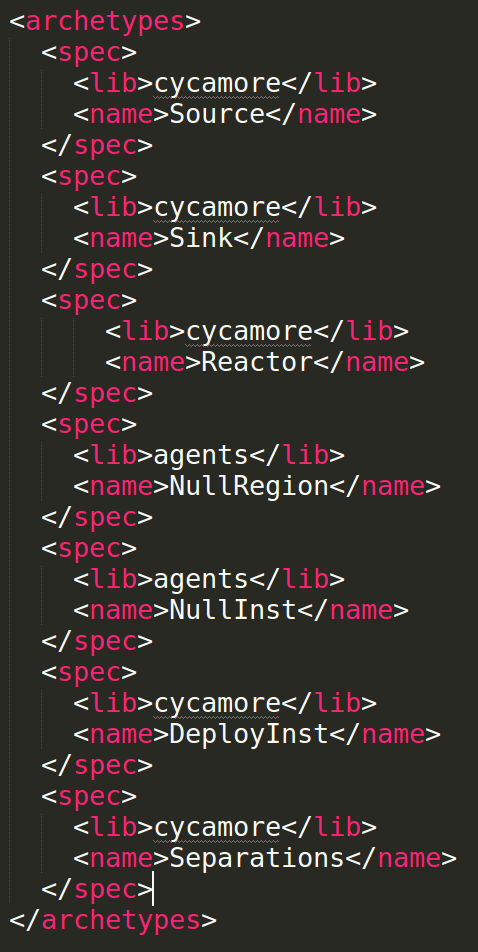
\includegraphics[height=.8\textheight]{./images/archetypes.png}
        \end{center}
    \end{figure}

\end{frame}

\begin{frame}
    \frametitle{Facility - Cycamore::Separations}
\begin{figure}[htbp!]
        \begin{center}
                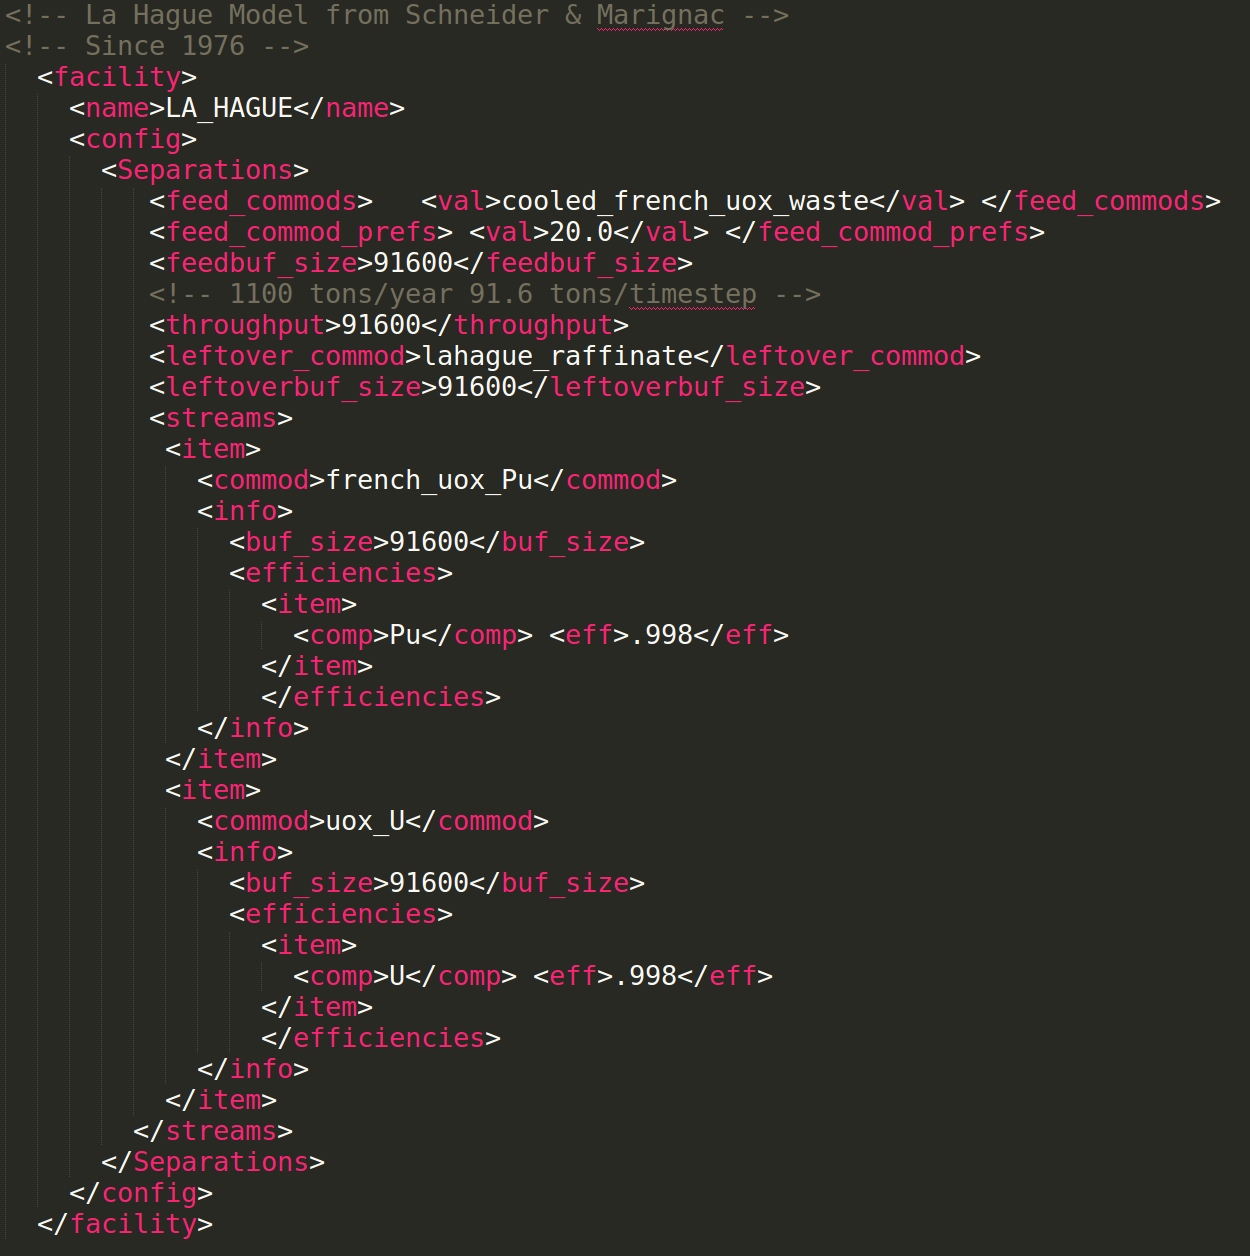
\includegraphics[width=.7\textwidth]{./images/lahague.png}
        \end{center}
    \end{figure}

\end{frame}

\begin{frame}
    \frametitle{Facility - Cycamore::Reactor}
\begin{figure}[htbp!]
        \begin{center}
                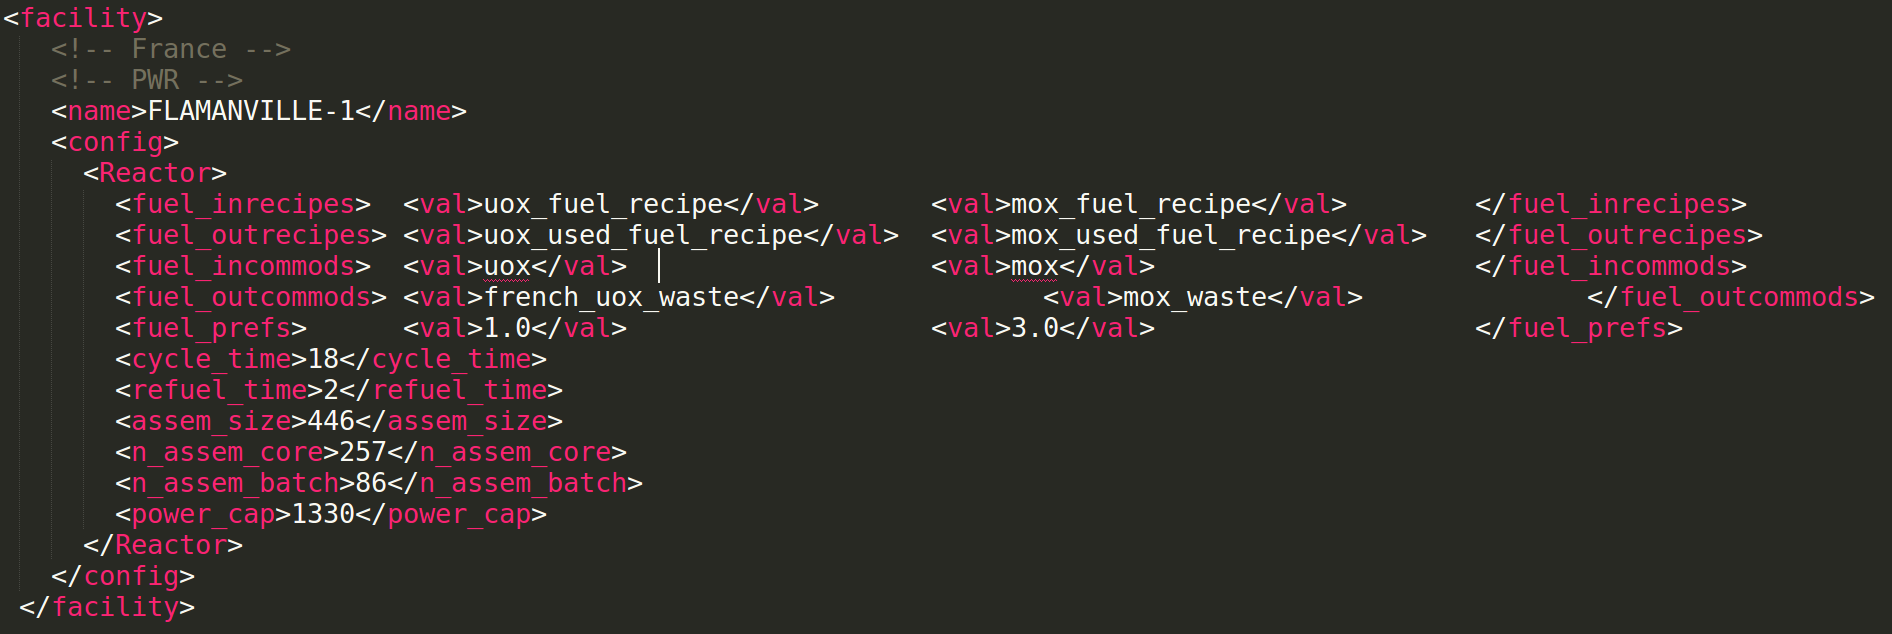
\includegraphics[width=1.1\textwidth]{./images/flamanville.png}
        \end{center}
    \end{figure}

\end{frame}

\begin{frame}
    \frametitle{Region}
\begin{figure}[htbp!]
        \begin{center}
                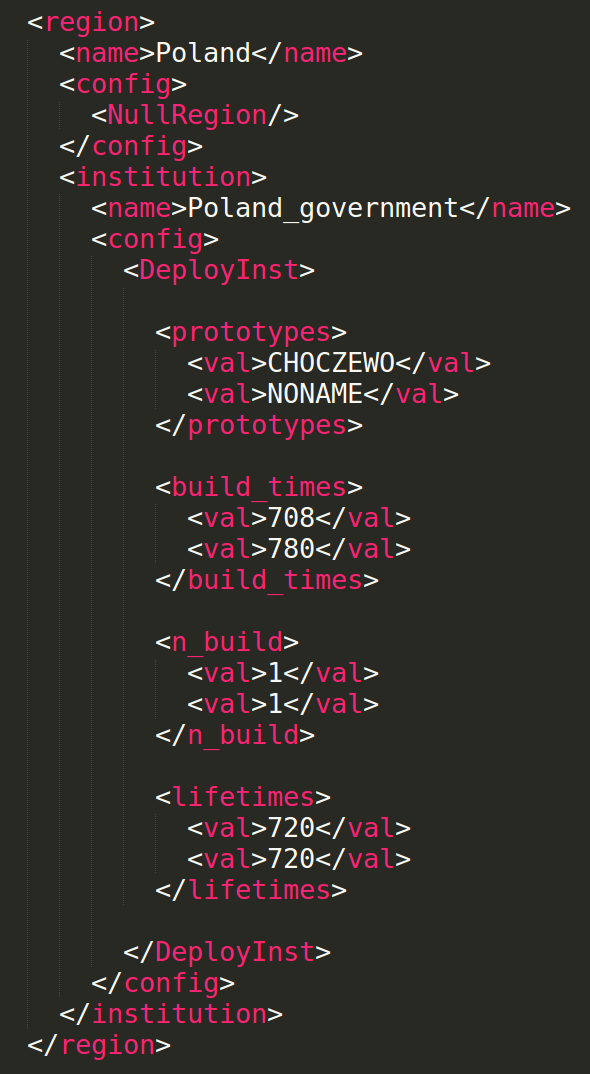
\includegraphics[height=.8\textheight]{./images/region.png}
        \end{center}
    \end{figure}

\end{frame}

\begin{frame}
    \frametitle{Recipe}
\begin{figure}[htbp!]
        \begin{center}
                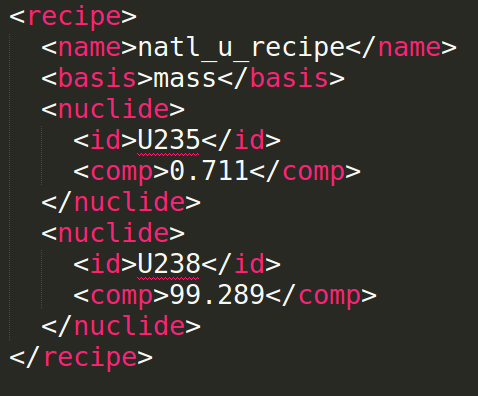
\includegraphics[width=.8\textwidth]{./images/recipe.png}
        \end{center}
    \end{figure}
\end{frame}


\begin{frame}
    \frametitle{Benefits}
    \begin{enumerate}
        \item Generate input file from database
        \begin{itemize}
            \item Reactor specifications from database
            \item Recipe from database
            \item Sensitivity study using external driver (e.g. RAVEN)
        \end{itemize}
        \item Simple automation / modification of input file
    \end{enumerate}
\end{frame}



\section{Output and Examples}
\begin{frame}
    \frametitle{Output}
    Cyclus records all transactions between \texttt{Facilities}
    and other metrics unique to each archetype, such as:
    \begin{itemize}
        \item Cycamore::Reactor - Power generation per timestep
        \item Cycamore::Enrichment - SWU per timestep
    \end{itemize}
\end{frame}


\subsection{Example - French Transition}
\begin{frame}
    \frametitle{Example Workflow}
    This workflow was used in the paper \texttt{Synergistic Spent Nuclear Fuel Dynamics Within the European Union} (in ANS 2017 Winter meeting, journal publication pending).

\begin{figure}
\scalebox{0.65}{
        \centering
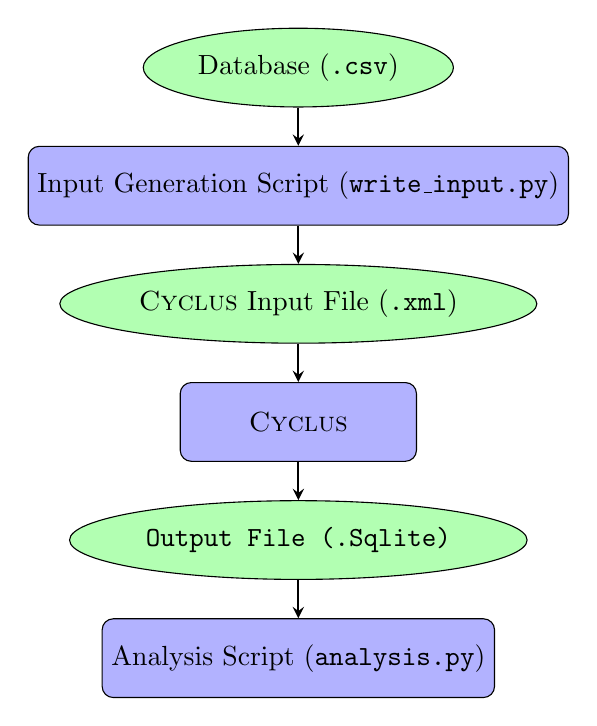
\begin{tikzpicture}[node distance=1.5cm]
\node (database) [object] {Database (\texttt{.csv})};
\node (script) [process, below of=database] {Input Generation Script (\texttt{write\_input.py})};
\node (input) [object, below of=script] {\Cyclus Input File (\texttt{.xml})};
\node (cyclus) [process, below of=input]{\Cyclus};
\node (output) [object, below of=cyclus]{\texttt{Output File (\texttt{.Sqlite})}};
\node (script2) [process, below of=output]{Analysis Script (\texttt{analysis.py})};

\draw [arrow] (database) -- (script); 
\draw [arrow] (script) -- (input); 
\draw [arrow] (input) -- (cyclus);
\draw [arrow] (cyclus) -- (output);
\draw [arrow] (output) -- (script2);
\end{tikzpicture}
}
\caption{Green circles and blue boxes represent files and software 
processes, respectively, in the computational workflow.}
\label{diag:comp}
\end{figure}

\end{frame}

\begin{frame}
    \frametitle{CSV to Cyclus input file}
    \begin{enumerate}
        \item Python script to parse through CSV file (reactor name, start / decom date, power output, etc)
        \item Use Jinja template to construct input file (Python script fills curly brackets)
    \end{enumerate}
    \begin{figure}[htbp!]
        \begin{center}
                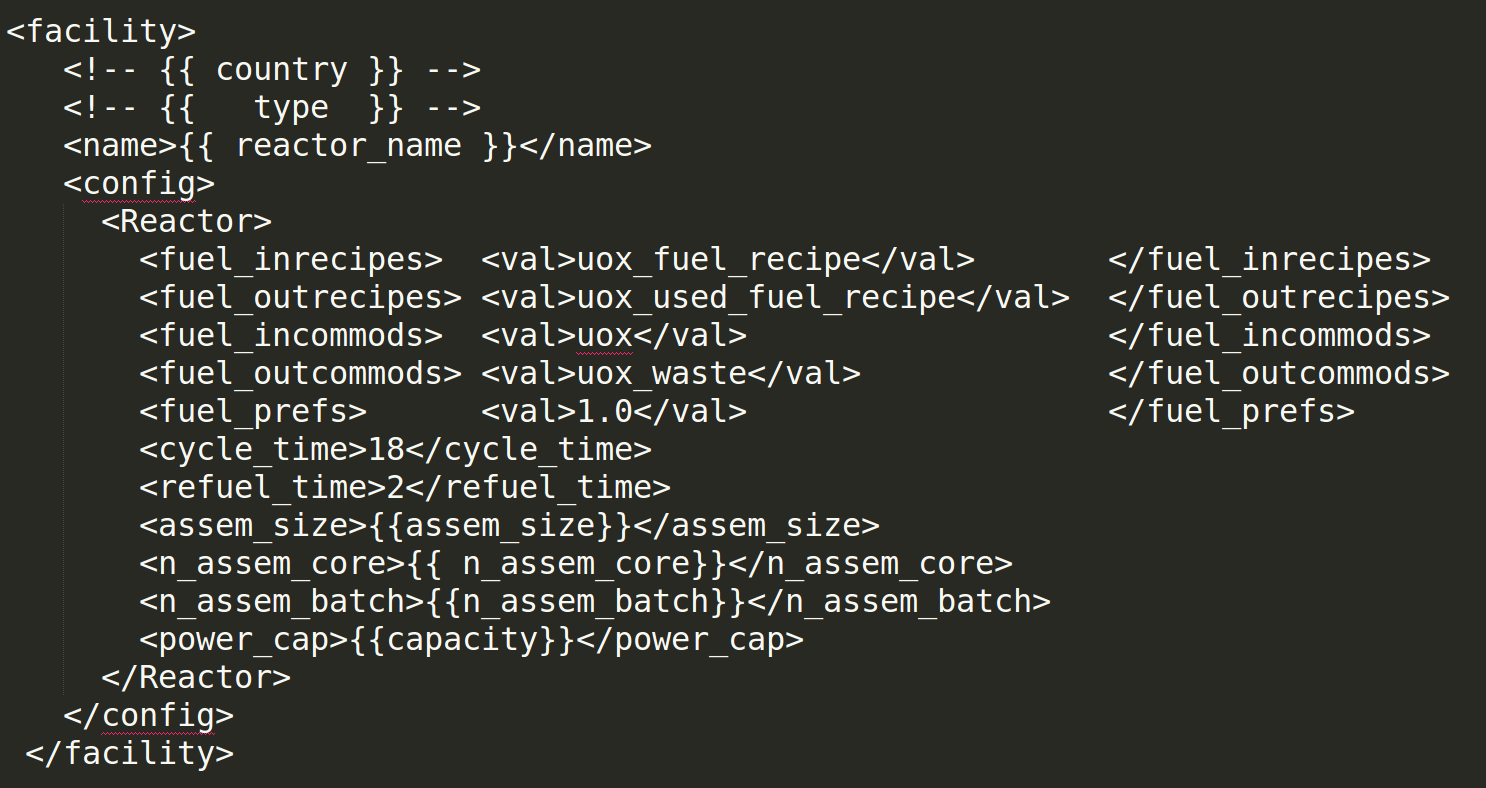
\includegraphics[width=.8\textwidth]{./images/reactor_template.png}
        \end{center}
    \end{figure}
\end{frame}

\begin{frame}
    \frametitle{Output analysis}
    \begin{itemize}
        \item Python script to query and process output data
        \item Use Jupyter notebook to organize / visualize output
    \end{itemize}

\end{frame}

\begin{frame}
    \frametitle{Output - regional analysis}
    \begin{itemize}
        \item The user can separate analysis by regions
        \item Concept of children-parent: each \texttt{facility} has a parent \texttt{Institution}, and each \texttt{Institution} has a parent \texttt{Region}.
    \end{itemize}
    \begin{figure}[htbp!]
        \begin{center}
                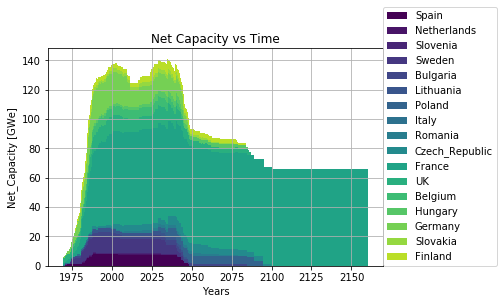
\includegraphics[width=.8\textwidth]{./images/sim_output/france/onesim.png}
        \end{center}
    \caption{Power generation is separated by region.}
    \end{figure}
\end{frame}

\begin{frame}
    \frametitle{Output - regional analysis}
    \begin{itemize}
        \item The user can separate analysis by regions
        \item Concept of children-parent: each \texttt{facility} has a parent \texttt{Institution}, and each \texttt{Institution} has a parent \texttt{Region}.
    \end{itemize}
    \begin{figure}[htbp!]
        \begin{center}
                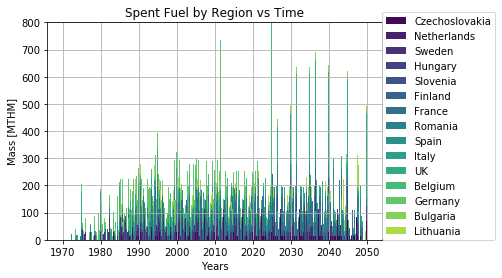
\includegraphics[width=.8\textwidth]{./images/sim_output/france/regional_snf.png}
        \end{center}
    \caption{Waste output mass is separated by their origin region.}
    \end{figure}
\end{frame}

\begin{frame}
    \frametitle{Output - Prototype analysis}
    \begin{itemize}
        \item The user can separate analysis by prototype
        \item User can see how much \texttt{power} is from SFRs compared to PWRs.
    \end{itemize}
    \begin{figure}[htbp!]
        \begin{center}
                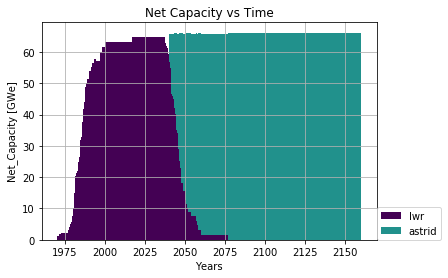
\includegraphics[width=.8\textwidth]{./images/sim_output/france/power_plot.png}
        \end{center}
    \caption{Power generation is separated by prototype (SFR, PWR).}
    \end{figure}
\end{frame}


\begin{frame}
    \frametitle{Output - Prototype analysis}
    \begin{itemize}
        \item The user can separate analysis by prototype
        \item User can see how much fuel is from which facility.
    \end{itemize}
    \begin{figure}[htbp!]
        \begin{center}
                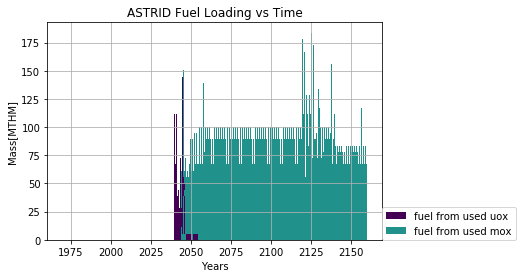
\includegraphics[width=.8\textwidth]{./images/sim_output/france/where_fuel.png}
        \end{center}
    \caption{Fuel production is separated by production facility.}
    \end{figure}
\end{frame}

\begin{frame}
    \frametitle{Sensitivity Study}
    Breeding ratio sensitivity study can be done by simply changing the 
    SFR output fuel recipe in the input file.
    \begin{figure}[htbp!]
        \begin{center}
                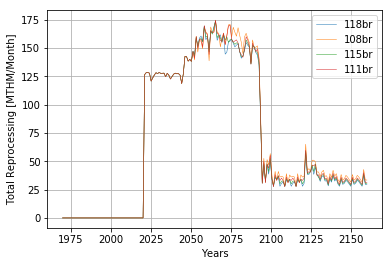
\includegraphics[width=.8\textwidth]{./images/sim_output/france/br_tot_rep.png}
        \end{center}
    \caption{Breeding Ratio affect on total reprocessing.}
    \end{figure}
\end{frame}

\begin{frame}
    \frametitle{Sensitivity Study}
    Lifetime extension sensitivity study can be done by adding the
    lifetime of the pwrs and adjusting SFR deployment accordingly.
    \begin{figure}[htbp!]
        \begin{center}
                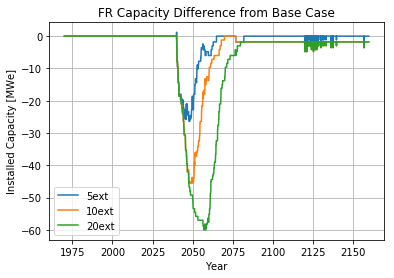
\includegraphics[width=.8\textwidth]{./images/sim_output/france/fr_diff.png}
        \end{center}
    \caption{PWR lifetime extension affect on FR installed capacity.}
    \end{figure}
\end{frame}




\subsection{Example - Predicting the past (U.S.)}

\begin{frame}
    \frametitle{Predicting the past - U.S}
    Work done by undergraduate researcher Gyutae Park at the University of Illinois - Urbana Champaign.
    \begin{enumerate}
        \item Import database to construct Cyclus simulation
        \item `Predict the past' - fuel usage, power generated
        \item Demonstrate GIS capabilities of Cyclus
    \end{enumerate}
\end{frame}


\begin{frame}
    \frametitle{Example Workflow}
    Similar workflow has been used for this analysis study.
\begin{figure}
\scalebox{0.65}{
        \centering
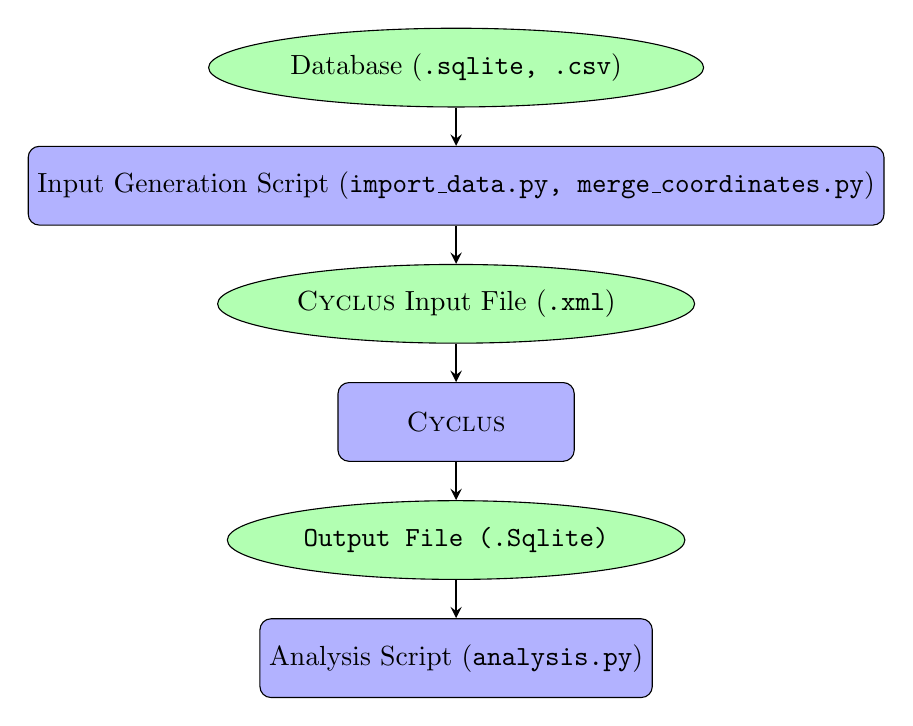
\begin{tikzpicture}[node distance=1.5cm]
\node (database) [object] {Database (\texttt{.sqlite, .csv})};
\node (script) [process, below of=database] {Input Generation Script (\texttt{import\_data.py, merge\_coordinates.py})};
\node (input) [object, below of=script] {\Cyclus Input File (\texttt{.xml})};
\node (cyclus) [process, below of=input]{\Cyclus};
\node (output) [object, below of=cyclus]{\texttt{Output File (\texttt{.Sqlite})}};
\node (script2) [process, below of=output]{Analysis Script (\texttt{analysis.py})};

\draw [arrow] (database) -- (script); 
\draw [arrow] (script) -- (input); 
\draw [arrow] (input) -- (cyclus);
\draw [arrow] (cyclus) -- (output);
\draw [arrow] (output) -- (script2);
\end{tikzpicture}
}
\caption{Green circles and blue boxes represent files and software 
processes, respectively, in the computational workflow.}
\label{diag:comp}
\end{figure}

\end{frame}

\begin{frame}
    \frametitle{Results - Fuel into reactors}
    \begin{figure}[htbp!]
        \begin{center}
                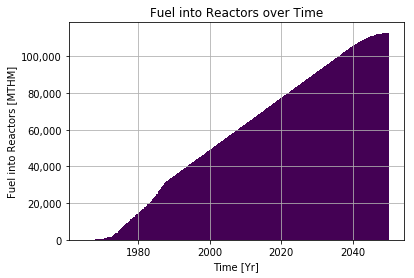
\includegraphics[width=.8\textwidth]{./images/sim_output/us/fuel.png}
        \end{center}
    \caption{Cumulative fuel into U.S. reactors over time.}
    \end{figure}
\end{frame}


\begin{frame}
    \frametitle{Results - Natural Uranium usage}
    \begin{figure}[htbp!]
        \begin{center}
                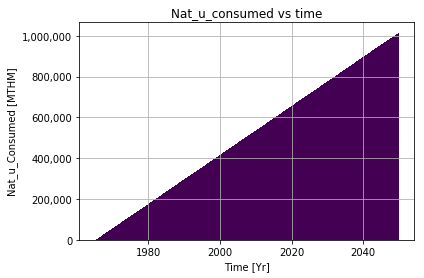
\includegraphics[width=.8\textwidth]{./images/sim_output/us/natu.png}
        \end{center}
    \caption{Cumulative natural uranium consumption in the U.S. over time.}
    \end{figure}
\end{frame}

\begin{frame}
    \frametitle{Results - Power generated}
\begin{figure}[htbp!]
\begin{minipage}[b]{.45\linewidth}
    \begin{center}
        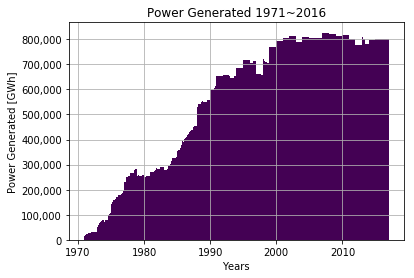
\includegraphics[width=\textwidth]{./images/sim_output/us/cyc_pow.png}
    \end{center}
    \caption{Nuclear Power generated simulated by Cyclus}
\end{minipage}
\hspace{.5cm}
\begin{minipage}[b]{.45\linewidth}
    \centering
        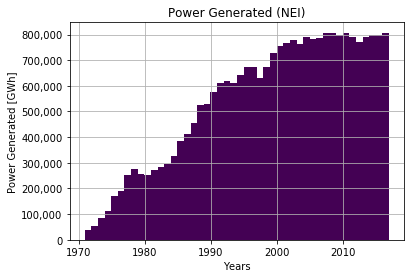
\includegraphics[width=\linewidth]{./images/sim_output/us/nei_pow.png}
    \caption{Nuclear power generation data from NEI \footnotemark}
\end{minipage}
\end{figure}
    \footnotetext{US Nuclear Generating Statistics. (n.d.). Retrieved from https://www.nei.org/Knowledge-Center/Nuclear-Statistics/US-Nuclear-Power-Plants/US-Nuclear-Generating-Statistics}
\end{frame}

\begin{frame}
    \frametitle{Results - GIS}
    \begin{figure}[htbp!]
        \begin{center}
                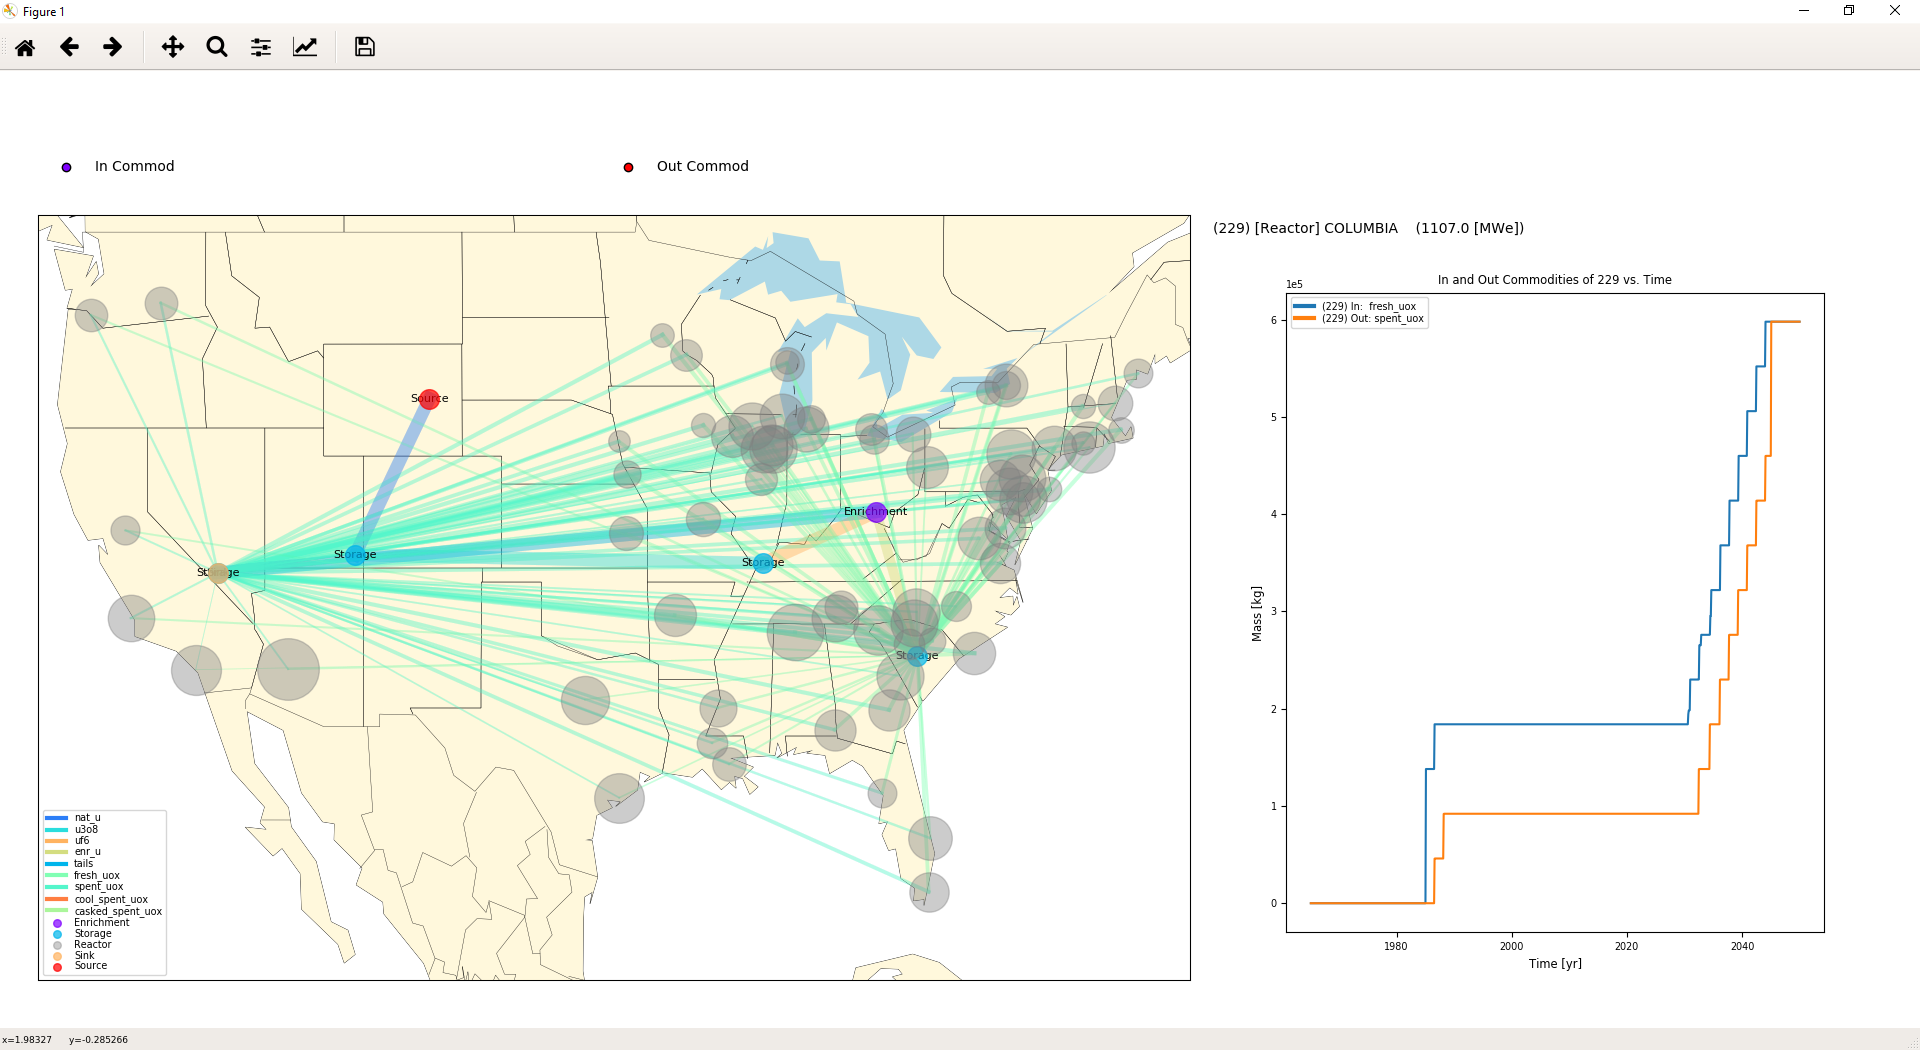
\includegraphics[width=.8\textwidth]{./images/sim_output/us/map.png}
        \end{center}
    \caption{Interactive map of U.S. reactors and fuel cycle
     facilities. Lines show transactions between two facilities.}
    \end{figure}
\end{frame}




\end{document}



